\documentclass[a0paper,fleqn]{betterposter}

%%%% Configuration (omitting most of the unused settings for brevity)

\renewcommand{\maincolumnbackgroundcolor}{theory}
\usepackage{caption}
\captionsetup{
	font=LARGE,       % set the font size to 'large' for both label and text
	labelfont=LARGE   % set the font size to 'large' for the label
}
\usepackage[square,numbers]{natbib}
%\usepackage[backend=biber, style=numeric, sorting=none]{biblatex}
\renewcommand{\bibfont}{\huge}

\usepackage{url}
%\usepackage{hyperref}

\begin{document}    
	\betterposter{
		%%%%%%%% SINGLE LEFT COLUMN (MERGED)
		
		\title{How do Bayesian Networks support impact-based forecasting for informed decision-making?}
		 \vspace{1em}%
		\section{
			\begin{minipage}[c]{0.07\textwidth}
				\includegraphics[width=\linewidth]{img/logo2.png}
			\end{minipage}%
		    \hspace{0.5em}%
			\begin{minipage}[c]{0.07\textwidth}
				\includegraphics[width=\linewidth]{img/logo1.png}
			\end{minipage}%
		    \hspace{1em}%
			\begin{minipage}[c]{0.9\textwidth}
				\underline{Nishadh Kalladath$^{1}$}, Viola Otieno$^{1}$, Jully Ouma$^{1,2}$, Collison Lorez${^1}$, \& Ahmed Amdihun${^1}$
				 \vspace{0.8em}%
				\\${^1}$ IGAD Climate Prediction and Applications Centre- ICPAC, Nairobi, Kenya
				\\${^2}$ United Nation Office for Disaster Risk Reduction, Africa Office, Kenya
			\end{minipage}
		}
	    \vspace{1em}%
		\hrule
		
		\section{Introduction}
	\begin{itemize}
		\item Impact-based forecasting (IBF) is pivotal for disaster risk management. It empowers decisions that anticipate and reduce damage and loss of life from natural hazards.
		\item IBF relies on risk matrices. These matrices evaluate probabilities or impact figures for specific events, such as floods. 
		\item However, they often miss out on considering conditional elements, potential interventions, and essential scenarios, especially the probable outcomes of different actions \cite{fenton2018risk}.
		\item Enter the Bayesian Network (BN): a directed graphical model that encapsulates variables and their conditional probabilistic interconnections.
	\end{itemize}
	
		
		\section{Methods}
		\begin{itemize}
			\item The figure \ref{fig1} illustrate the method for creating a BN model. This model can be broadened to include inputs and applications crucial for decision-making.
			\item The presented BN model leverages insights from GPT-4V using the Python library pgmpy.
		\end{itemize}
		\begin{center}
			%\begin{figure}[h!]	
			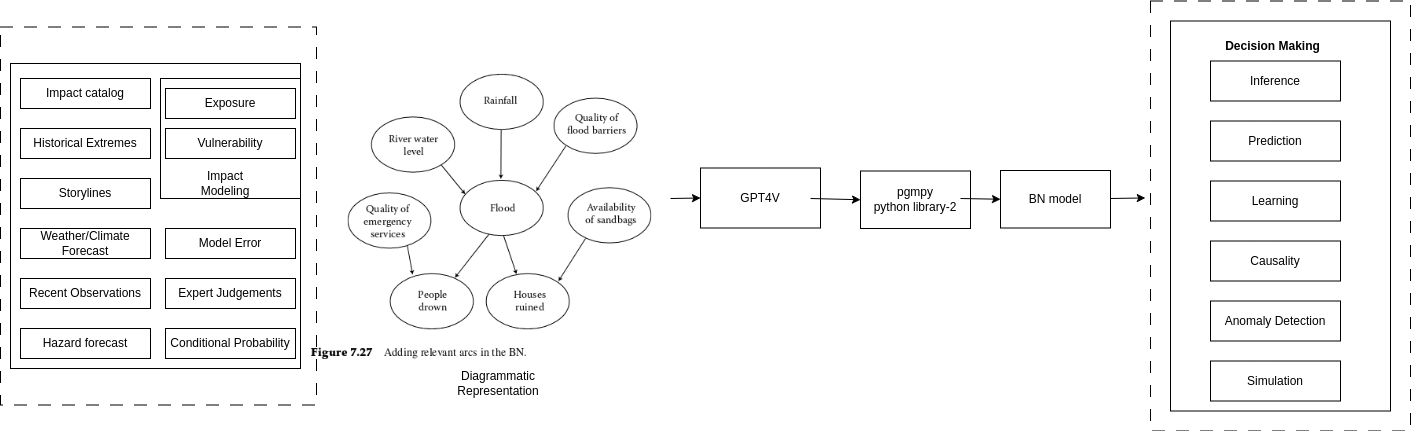
\includegraphics[width=\textwidth]{img/BN-model-IBF-v2.png}
			\captionof{figure}{Steps for BN generation using GPT-4V\cite{openai2023gpt4} and the Python library pgmpy\cite{ankan2015pgmpy}. The test image is adapted from \citet{fenton2018risk}.}
			\label{fig1}
			%\end{figure}
		\end{center}
		
		
	    \section{Results}
		\begin{itemize}
			\item Our Jupyter Notebook on GitHub provides preliminary findings on using BN for carry out analysis for antciaptory action against flood hazards. 
			\item We are expanding the study to widen the applications of our findings.
		\end{itemize}
		%% Institution logo
		%\includegraphics[width=\textwidth]{img/logo}\\
		\section{Reference}
		%\begin{enumerate}
		%\item 
		%\item OpenAI. "GPT-4 Technical Report." arXiv e-prints, 2023, arXiv:2303.08774.
		%\item Ankan, Ankur, and Abinash Panda. 2015. [4]. 
		%\item Ankan, Ankur, and Abinash Panda. 2015. [4] \LARGE{"pgmpy: Probabilistic graphical models using python." Proceedings of the 14th python in science conference (scipy 2015). Vol. 10. Citeseer, 2015.}
		%\item \url{github.com/nishadhka/bn-ibf/code/01-simple-bn-flood.ipynb }
		\renewcommand{\bibsection}{}                                                                                                               
		\bibliographystyle{unsrtnat} % or another suitable style like abbrvnat, unsrtnat, etc.
		\bibliography{references} % if your file is named references.bib
		%\printbibliography
		
	    %\end{enumerate}
		
		%\author{Mike Morrison}
		%\author{Rafael Bailo}
		%\institution{Optional Institution Under Name}
	}	
	{
		%%%%%%%% MAIN COLUMN
		\maincolumn{
			%%%% Main space
						
		Current IBF practices, lacking in addressing uncertainty, diverse views, and transparency, miss the 'skin in the game'\cite{taleb2018skin}. Integrating Bayesian Networks with GPT-4V/LLM could enhance IBF
			
		}{
			%%%% Bottom space
		\qrcode{img/qrcode-bn}{img/smartphoneWhite}{
			\textbf{Scan the QR Code} for \\ supporting materials
			\\ \textbf{@ GitHub Repository:}
			\\icpac-igad/bn-ibf
			\\ \textbf{For Comments \& Queries:}
			\\icpac-igad/bn-ibf/issues
		}
		}
		
	}
	
\end{document}
